% !TEX program = xelatex
\PassOptionsToPackage{no-math}{fontspec}
\documentclass[10pt,a4paper,fontset=fandol]{ctexart}

\usepackage[margin=2.1cm]{geometry}
\usepackage{amsmath,amsthm,amssymb}
\usepackage{fontspec}
\setmainfont{Liberation Serif}
\setsansfont{Liberation Sans}
\setmonofont[Scale=0.88]{Maple Mono NF CN}
\setCJKmonofont[Scale=0.88]{Maple Mono NF CN}

\usepackage{mathpartir}
\usepackage{stmaryrd}
\usepackage{booktabs}
\usepackage{xcolor}
\usepackage{tikz}
\usetikzlibrary{arrows.meta, positioning, fit, calc}
\usepackage{listings}
\usepackage[colorlinks=true,linkcolor=NavyBlue,citecolor=TealInk,urlcolor=TealInk]{hyperref}
\usepackage[capitalize,noabbrev]{cleveref}

\definecolor{NavyBlue}{HTML}{1B365D}
\definecolor{TealInk}{HTML}{2B6CB0}
\definecolor{ForestInk}{HTML}{276749}
\definecolor{AmberInk}{HTML}{B7791F}
\definecolor{TintBlue}{HTML}{EDF4FC}
\definecolor{TintNavy}{HTML}{F4F7FA}
\definecolor{TintAmber}{HTML}{FEFBF3}
\definecolor{TintGreen}{HTML}{F2FBF6}

\lstdefinelanguage{LeanFour}{
  morekeywords={import,namespace,end,def,theorem,lemma,Prop,Type,let,do,for,in,if,then,else,return,open,section,private,where,match,with},
  sensitive=true,
  morecomment=[l]{--},
  morecomment=[n]{/-}{-/},
  morestring=[b]"
}

\lstset{
  basicstyle=\ttfamily\footnotesize,
  keywordstyle=\bfseries\color{NavyBlue},
  commentstyle=\itshape\color{gray},
  columns=fullflexible,
  keepspaces=true,
  aboveskip=5pt,
  belowskip=5pt
}

\newtheorem{theorem}{定理}[section]
\newtheorem{definition}[theorem]{定义}
\renewcommand{\proofname}{证明}

\crefname{section}{第}{第}
\Crefname{section}{第}{第}
\creflabelformat{section}{#2#1#3 节}
\crefname{theorem}{定理}{定理}
\Crefname{theorem}{定理}{定理}
\crefname{definition}{定义}{定义}
\Crefname{definition}{定义}{定义}
\crefname{figure}{图}{图}
\Crefname{figure}{图}{图}
\crefname{table}{表}{表}
\Crefname{table}{表}{表}

% Notation macros (identical to EN paper)
\newcommand{\Cinfra}{\mathcal{C}_{\mathrm{infra}}}
\newcommand{\Truth}{\mathcal{E}}
\newcommand{\Orch}{\mathcal{G}}
\newcommand{\Ledger}{\mathcal{L}}
\newcommand{\Events}{\Lambda}
\newcommand{\Spec}{\mathrm{Spec}}
\newcommand{\Prop}{\mathsf{Prop}}
\newcommand{\TypeU}{\mathsf{Type}\;u}
\newcommand{\DefEq}{\equiv_{\beta\delta\iota\zeta}}
\newcommand{\AxiomsZero}{\mathcal{A}_0}
\newcommand{\judge}[3]{#1 \vdash_{\mathrm{accept}} #2 \Downarrow #3}
\newcommand{\irstep}[4]{#1 \xrightarrow{#2}_{#3} #4}
\newcommand{\kw}[1]{\mathsf{#1}}
\newcommand{\code}[1]{\texttt{#1}}
\emergencystretch=2em

\title{\textbf{作为并发边界的证明无关性：}\\
\large 协作式依赖类型定理证明中真值、核验与编排的解耦机制}

\author{Quod 架构工作组\\
\small Quod Project（英文原版：\code{quod-core-mechanisms.pdf}）}
\date{}

\begin{document}
\maketitle

\begin{abstract}
依赖类型论（尤其是 Lean~4 所采用的归纳构造演算，CIC）下的大规模协作形式化，在“多智能体并发搜索”与“基础逻辑可靠性（Soundness）”之间存在根本张力。与经典一阶逻辑不同，朴素的与或（AND-OR）证明搜索超图在 Lean~4 的依赖类型体系下会直接失效：对 $\TypeU$ 中的存在性构造进行拆分，会因 $\TypeU$ 不满足证明无关性（Proof Irrelevance）而产生无法合流的见证元（witness）冲突；而辅助定义、结构体与类型类实例也无法编码为纯命题超边。更严重的是，若将大语言模型（LLM）嵌入证明编排器或核验回路，会直接污染可信计算基（TCB）。

本文对事件溯源、零内置 LLM 的 Lean~4 协作验证设施 \textsc{Quod} 的核心机制给出形式化刻画。\textsc{Quod} 通过三项紧耦合的机制化解上述张力：
（1）\textbf{真值层与编排层的正交解耦}：将系统状态拆分为单调、内容寻址的 \emph{Verified Overlays} 真值层与非单调的 \code{Route} 分组任务有向无环图（DAG），并强制所有面向 Worker 的义务均为闭合 $\Prop$（从而以 CIC 的证明无关性作为无锁竞速的并发边界）；
（2）\textbf{零 LLM 极小可信计算基（$\Cinfra$）与分层核验语义}：通过静态 Stage~0 卫生与最小导入门禁、\code{bwrap} 隔离的 Stage~1 Lean~4 内核定义等价（\code{isDefEq}）与公理闭包审计、职责分离以及与内核验收绑定的积分结算确保可靠；
（3）\textbf{封闭代数编排中间表示（\code{GraphIrOp}）与三时间尺度 $(E, C, I)$ 效应隔离}：在事件溯源有限状态机上执行受限声明式原语，并以投影过滤跨尺度信息流。
我们形式化给出了上述机制的操作语义，并证明了编排--可靠性非干扰定理、竞速胜者无关性定理、相对内核可靠性定理与事件重放单调性定理。
\end{abstract}

% =========================================================
\section{引言与动机示例}\label{sec:intro}
% =========================================================

大规模形式化数学正越来越依赖人类数学家与异构自动证明器或 LLM 编码智能体的并行协作~\cite{demoura2021lean4,mathlib2020}。然而，现有的绝大多数智能体证明框架都将证明器外壳（harness）设计成单体结构：LLM 循环生成策略（tactic）、调用 Lean、解析原始编译器报错、直接改写共享文件并维护临时性的证明图。一旦推广到开放、多参与者协作场景，这种单体模型会暴露出三类结构性缺陷：

\begin{enumerate}
  \item \textbf{依赖类型拆分困境。} 在 Lean~4 的归纳构造演算（CIC）中，证明无关性仅对 $\Prop$（\code{Sort 0}）成立，对计算宇宙 $\TypeU$（\code{Sort (u+1)}）则\emph{不成立}。若协调器将 $\exists w : \alpha,\, P(w) \land Q(w)$ 拆分为“构造满足 $P(w_1)$ 的 $w_1 : \alpha$”与“构造满足 $Q(w_2)$ 的 $w_2 : \alpha$”两个并发子目标，当不同 Worker 给出 $w_1 \not\DefEq w_2$ 时，下游合并必然失败。此外，数学工程高度依赖非命题声明（\code{def}、\code{structure}、\code{instance}、\code{@[simp]}），它们无法表示为纯命题图边。
  \item \textbf{TCB 膨胀与规范漂移。} 将 LLM 启发式或外部 Worker 提供的元数据放入验收路径，会引入通过注入 \code{axiom}、\code{sorry}、\code{native\_decide}、元编程（\code{elab}、\code{macro\_rules}）、IO 后门或规范漂移（包括空真定理陈述）破坏可靠性的风险。
  \item \textbf{上下文污染与图结构破坏。} 将原始 Lean 报错栈灌入战略编排器会严重劣化推理质量，而允许未授权 Worker 任意改写全局任务图则会诱发刷图与算力浪费。
\end{enumerate}

\textsc{Quod}（\emph{Quod Erat Demonstrandum}）将平台本身定位为\textbf{零内置 LLM 的确定性设施（$\Cinfra$）}，把\textbf{机制}（可靠性、身份权限、状态迁移与署名记账）与\textbf{策略}（拆题、定价与证明搜索）彻底分离。

\paragraph{贯穿示例。}
本文以 \textsc{Quod} 的 Erd\H{o}s 第 479 问题规范（\code{examples/erdos-479/Quod/Epoch1/Spec.lean}）作为贯穿示例：
\begin{lstlisting}[language=LeanFour]
import Mathlib.Data.Int.ModEq
import Mathlib.Data.Set.Finite.Basic
namespace Quod.Epoch1
def erdos_479_stmt : Prop :=
  forall k : Int, k != 1 ->
    { n : Nat | (2 : Int) ^ n == k [ZMOD (n : Int)] }.Infinite
end Quod.Epoch1
\end{lstlisting}
这段仅 11 行的规范体现了两个刻意坚守的不变量：（i）根目标 \code{erdos\_479\_stmt} 是类型为 $\Prop$ 的闭合项；（ii）规范采用最小精细导入而非全量 \code{import Mathlib}，从而避免端侧参与者在有限内存下发生严重交换抖动，并保证沙箱核验的敏捷性。

\paragraph{本文贡献与边界说明。}
本文的贡献直接锚定于 \textsc{Quod} 的 Rust 核心实现（\code{quod-core}、\code{quod-sandbox}、\code{quod-verifier}、\code{quod-store}、\code{quod-hub}）：
\begin{itemize}
  \item \textbf{机制 A（\Cref{sec:mech-a}）：} 形式化 \textsc{Quod} 将状态正交解耦为单调 \emph{Verified Overlays} 真值层（$\Truth$）与非单调 \code{Route} 分组任务 DAG（$\Orch$）的双层结构，以及面向 Worker 的闭合 $\Prop$ 统一协议，并证明\emph{编排--可靠性非干扰定理}（\Cref{thm:non-interference}）与\emph{竞速胜者无关性定理}（\Cref{thm:race-irrelevance}）。
  \item \textbf{机制 B（\Cref{sec:mech-b}）：} 刻画零 LLM 极小 TCB（$\Cinfra$）的分层操作语义，涵盖 Stage~0 静态卫生门禁、Stage~1 \code{bwrap} 隔离下的 Lean~4 内核 \code{isDefEq} 与公理闭包审计、职责分离以及原子积分结算，并证明\emph{相对内核可靠性定理}（\Cref{thm:kernel-soundness}）与\emph{零自报积分完整性定理}（\Cref{thm:credit-integrity}）。
  \item \textbf{机制 C（\Cref{sec:mech-c}）：} 对封闭代数编排语言 \code{GraphIrOp} 与三时间尺度 $(E, C, I)$ 下的事件溯源有限状态机（\code{Epoch}、\code{Task}、\code{Submission}）建模，建立\emph{事件重放确定性与真值单调性定理}（\Cref{thm:replay}）及\emph{合并任务依赖注入完备性定理}（\Cref{thm:merge-unlock}）。
\end{itemize}
\Cref{sec:impl} 将上述形式化语义映射至 Rust 工作区，并清晰区分当前已实现核心与文档中规划的架构扩展（L5 可达性剪枝/Git 重放与 M4 在线 IRT 校准）。

% =========================================================
\section{系统模型：三时间尺度 $(E, C, I)$ 分离}\label{sec:model}
% =========================================================

\textsc{Quod} 沿两条正交轴组织协作：\textbf{信任与能动性分层} $(E, C, I)$ 与\textbf{运行时间尺度}（$\kw{Scale\;0}, \kw{Scale\;1}, \kw{Scale\;2}$）。

\begin{itemize}
  \item \textbf{环境 / 状态层（$E$）：} 持久化的数学制品、任务图、只追加事件日志与积分账本（$E_0, E_1, E_2$）。
  \item \textbf{确定性设施层（$C$）：} 构成 $\Cinfra$ 的零 LLM Rust 服务与 Lean~4 核验沙箱（$C_0, C_1, C_2$）。$C$ 层\emph{不包含}任何大模型调用、启发式推理或自主循环。
  \item \textbf{人机同构外部智能层（$I$）：} 人类数学家与外部 AI 智能体作为同构的认证 \code{Actor} 接入（$I_0$ Worker、$I_1$ Orchestrator、$I_2\text{-B}$ Blueprinter、$I_2\text{-A}$ Auditor）。
\end{itemize}

\begin{table}[t]
\centering
\caption{\textsc{Quod} 中的三时间尺度 $(E, C, I)$ 分层架构。}
\label{tab:eci}
\small
\begin{tabular}{@{}lp{3.7cm}p{4.1cm}p{3.6cm}@{}}
\toprule
\textbf{时间尺度} & \textbf{状态层（$E$）} & \textbf{确定性设施（$C$，0 LLM）} & \textbf{外部智能（$I$）} \\
\midrule
\textbf{Scale 0}（毫秒--分） &
$E_0$：\code{events}、CAS 源码库、租约、\code{.olean}、\code{credit\_ledger}、Graveyard &
$C_0$：\code{quod-hub} + \code{quod-verifier}、Ed25519 RBAC、Stage~0/1、原子结算 &
$I_0$（\code{Worker}）：本地证明/反驳搜索、\code{fetch}/\code{submit} \\
\addlinespace
\textbf{Scale 1}（分--小时） &
$E_1$：\code{Verified Overlays} + \code{Route} 分组 $\Prop$ DAG + 遥测摘要 &
$C_1$：\code{GraphIrOp} 校验解释器、\code{WakeupDigest}、\code{quod-algo} &
$I_1$（\code{Orchestrator}）：开辟/剪枝 \code{Route}、拆题、悬赏定价 \\
\addlinespace
\textbf{Scale 2}（天--周） &
$E_2$：\code{Project} 名录、不可变 \code{Epoch} \code{Spec}、共享工具链包 &
$C_2$：最小导入与 SHA-256 门禁、Epoch FSM、（扩展：L5 导出） &
$I_2\text{-B}$（\code{Blueprinter}）与 $I_2\text{-A}$（\code{Auditor}） \\
\bottomrule
\end{tabular}
\end{table}

\paragraph{人机同构鉴权与 RBAC。}
每位参与者（无论人类或智能体）均注册一对 Ed25519 公钥 $pk_a$，绑定至 \code{ActorAuthContext} $(a, \kw{roles}_a, \kw{scopes}_a, \kw{enabled}_a)$，其中 $\kw{roles}_a \subseteq \{\kw{Worker}, \kw{Orchestrator}, \kw{Blueprinter}, \kw{Auditor}, \kw{Admin}\}$。所有写操作 HTTP 请求 $(m, p, \tau, b)$ 均携带头信息 $(a, \tau, \sigma)$，在 $C_0$ 内按规范签名载荷验签：
\[
\kw{payload}(m, p, \tau, b) = \kw{upper}(m) \,\|\, \text{\code{"\textbackslash n"}} \,\|\, p \,\|\, \text{\code{"\textbackslash n"}} \,\|\, \tau \,\|\, \text{\code{"\textbackslash n"}} \,\|\, \kw{SHA256}(b),
\]
同时硬性校验时间戳偏差 $|\tau_{\mathrm{now}} - \tau| \le \Delta_{\max}$、角色权限与项目作用域（$\kw{scopes}_a = \emptyset$ 表示全局域，否则要求 $pid \in \kw{scopes}_a$）。授权委派同样分层锁死：\code{Blueprinter} 仅能在其 \code{project\_scopes} 内签发 \code{Worker} 或 \code{Orchestrator} 邀请码，而 \code{Auditor}、\code{Admin} 与全局作用域必须由 \code{Admin} 签发。

\begin{figure}[t]
\centering
\begin{tikzpicture}[
  x=1cm, y=1cm,
  boxI/.style={rectangle, rounded corners=3pt, draw=TealInk, fill=TintBlue, font=\sffamily\footnotesize, align=center, inner sep=5pt, minimum width=2.8cm, minimum height=0.85cm},
  boxC/.style={rectangle, rounded corners=3pt, draw=NavyBlue, thick, fill=TintNavy, font=\sffamily\footnotesize, align=center, inner sep=5pt, minimum width=3.1cm, minimum height=0.85cm},
  boxE/.style={rectangle, rounded corners=3pt, draw=AmberInk, fill=TintAmber, font=\sffamily\footnotesize, align=center, inner sep=5pt, minimum width=3.0cm, minimum height=0.85cm},
  arr/.style={-{Stealth[length=4.5pt]}, line width=0.75pt, draw=NavyBlue},
  darr/.style={<-{Stealth[length=4.5pt]}, line width=0.75pt, draw=TealInk}
]
\node[boxI] (I2) at (0, 2.5) {$I_2$-B / $I_2$-A\\{\scriptsize 规范提案与独立审计}};
\node[boxC] (C2) at (4.0, 2.5) {$C_2$ 纪元门禁\\{\scriptsize SHA-256 / 职责分离}};
\node[boxE] (E2) at (8.1, 2.5) {$E_2$ 规范与共享缓存\\{\scriptsize 不可变 Epoch}};

\node[boxI] (I1) at (0, 1.25) {$I_1$ 编排者\\{\scriptsize 仅读摘要 Digest}};
\node[boxC] (C1) at (4.0, 1.25) {$C_1$ Graph IR 门禁\\{\scriptsize 封闭 DSL + \code{algo}}};
\node[boxE] (E1) at (8.1, 1.25) {$E_1$ Overlays $\oplus$ DAG\\{\scriptsize 真值层 $\perp$ 编排层}};

\node[boxI] (I0) at (0, 0.0) {$I_0$ 外部 Worker\\{\scriptsize 仅限闭合 \code{Prop}}};
\node[boxC] (C0) at (4.0, 0.0) {$C_0$ Hub + Verifier\\{\scriptsize Stage 0/1 + 积分账本}};
\node[boxE] (E0) at (8.1, 0.0) {$E_0$ 事件与 CAS 存储\\{\scriptsize \code{.olean} + Credits}};

\draw[arr] (I2) -- (C2);
\draw[darr] (C2) -- (E2);
\draw[darr] (I1) -- (C1);
\draw[darr] (C1) -- (E1);
\draw[arr] (I0) -- (C0);
\draw[darr] (C0) -- (E0);

\draw[arr] (C2) -- (C1);
\draw[arr] (C1) -- (C0);
\draw[arr] (E0) -- (E1);
\draw[arr] (E2) -- (E1);

\draw[dashed, NavyBlue!70, rounded corners=4pt] (2.25, -0.58) rectangle (5.75, 3.05);
\node[anchor=south, font=\sffamily\scriptsize\bfseries, text=NavyBlue] at (4.0, 3.06) {可信计算基 TCB（$\Cinfra$，0 LLM）};
\end{tikzpicture}
\caption{$(E, C, I)$ 与三时间尺度下的权限流向及 TCB 边界。}
\label{fig:eci}
\end{figure}

% =========================================================
\section{机制 A：真值层与编排层的正交解耦}\label{sec:mech-a}
% =========================================================

本节形式化说明：将 $E_1$ 拆分为只增不改的真值层与可变的编排层，并强制所有 Worker 任务均为闭合 $\Prop$，如何从构造上保障并发证明搜索的可靠性。

\subsection{为什么朴素超图在 CIC 中会失效？}
考虑构造性存在规范 $\exists w : \alpha,\, P(w) \land Q(w)$。若朴素与或超图将其拆为“构造满足 $P(w_1)$ 的 $w_1 : \alpha$”与“构造满足 $Q(w_2)$ 的 $w_2 : \alpha$”两个并行 Worker 任务，下游能否合并完全取决于 $w_1 \DefEq w_2$ 是否成立——一旦两个 Worker 选出不同见证元即宣告失败。同理，若 $P(w)$ 与 $Q(w)$ 共享某个 $\TypeU$ 对象 $w : \alpha$，则在两个引理通过类型检查前就必须先将非命题 \code{def} 注入 Lean 环境。因此，\textbf{真值累积}（单调扩展 Lean \code{Environment}）与\textbf{证明搜索编排}（提出、调权与剪枝子目标）本质上是两类完全不同的代数结构。

\subsection{双层状态分解}

\begin{definition}[单调真值层 $\Truth$]\label{def:truth-layer}
给定项目 $pid$ 与活跃纪元 $e$，真值层（\emph{Verified Overlays}）是一个有限偏映射 $\Truth : \kw{ModName} \rightharpoonup \kw{OverlayEntry}$，其中每个条目 $(k, \kw{src}, \kw{olean}, h, \kw{imps})$ 包含叠加层类型 $k \in \{\kw{Spec},\allowbreak \kw{DefOverlay},\allowbreak \kw{ProvedTask}\}$、UTF-8 源码 $\kw{src}$、编译后的 \code{.olean} 二进制制品、内容哈希 $h = \kw{SHA256}(\kw{src})$ 以及声明依赖 $\kw{imps} \subseteq \mathrm{dom}(\Truth)$。$\Truth$ 按单调扩展序偏序排列：
\[
\Truth \sqsubseteq \Truth' \iff \mathrm{dom}(\Truth) \subseteq \mathrm{dom}(\Truth') \land \forall m \in \mathrm{dom}(\Truth),\, \Truth'(m) = \Truth(m).
\]
进一步要求：每个模块 $m \in \mathrm{dom}(\Truth)$ 都必须在其声明的 $\kw{imps}$ 下由 Lean~4 零 \code{sorry} 编译通过，且所用公理严格落入允许集合 $\AxiomsZero$。
\end{definition}

\begin{definition}[非单调编排层 $\Orch$]\label{def:orch-layer}
编排层是一个由 \code{Route} 分组的有向无环图 $\Orch = (R, V, D_{\mathrm{dep}}, D_{\mathrm{ref}})$：
\begin{itemize}
  \item $R$ 为探索路线有限映射 $r \mapsto (\kw{title}, \kw{state}_r)$，其中 $\kw{state}_r \in \{\kw{Active}, \kw{Won}, \kw{Pruned}, \kw{Refuted}\}$；
  \item $V$ 为任务节点有限映射 $v \mapsto (\rho_v, \phi_v, I_v, s_v, \beta_v)$，其中：
    \begin{itemize}
      \item $\rho_v \in \{\kw{Root}, \kw{Lemma}, \kw{Connector}, \kw{Merge}, \kw{Refutation}, \kw{AuxLemma}, \kw{WitnessBundle}, \kw{Porting}\}$ 为战术角色；
      \item $\phi_v$ 是满足 $\Truth \vdash \phi_v : \Prop$ 的\emph{闭合}目标命题（引用锁定声明或内联 $\Prop$ 表达式）；
      \item $I_v \subseteq \mathrm{dom}(\Truth)$ 为节点携带的 \code{curated\_imports}；
      \item $s_v \in \kw{TaskState}$ 为生命周期状态；$\beta_v = (\kw{prio}_v, p_v, c_v, k_v, \kw{tier}_v, b_v)$ 保存调度与悬赏参数。
    \end{itemize}
  \item $D_{\mathrm{dep}} \subseteq V \times V$ 为保持无环的 \code{DependsOn} 依赖边，$D_{\mathrm{ref}} \subseteq V \times V$ 为 \code{Refutes} 反驳边。
\end{itemize}
\end{definition}

与 $\Truth$ 不同，$\Orch$ 是\emph{非单调}的：路线可以被剪枝、优先级与悬赏可随时调整、子目标可动态重组，但永远不会撤回或篡改 $\Truth$ 中已确认的模块。

\subsection{闭合 $\Prop$ 统一协议}
所有可被外部 Worker $I_0$ 认领的任务，100\% 均为闭合 $\Prop$ 义务。\Cref{tab:closed-prop} 归纳了各类协作语义如何统一编码为闭合 $\Prop$ 任务。

\begin{table}[t]
\centering
\caption{多种协作语义在 $\Orch$ 中的闭合 $\Prop$ 统一编码。}
\label{tab:closed-prop}
\small
\begin{tabular}{@{}ll@{}}
\toprule
\textbf{协作语义} & \textbf{在 $\Orch$ 中的闭合 $\Prop$ 表达} \\
\midrule
直接引理证明 & 目标 $\phi_v \equiv G : \Prop$（\code{Lemma} / \code{AuxLemma}） \\
反例证伪探针 & 目标 $\phi_v \equiv \neg P : \Prop$（\code{Refutation}） \\
拆解前充分性校验 & 目标 $\phi_v \equiv P_1 \to P_2 \to G : \Prop$（\code{Connector}） \\
跨路线等价桥接 & 目标 $\phi_v \equiv A \to B : \Prop$（\code{Lemma}） \\
存在耦合构造 & $\kw{Nonempty}\; B : \Prop$（\code{WitnessBundle}），或证得 $h_{\mathrm{ex}} : \exists w,\, \mathrm{Spec}\; w$ 后用 \code{Classical.choose} 解耦 \\
后置合并（合并即任务） & 目标 $\phi_v \equiv G : \Prop$，设 $\kw{depends\_on} = [P_1, P_2]$；$C_0$ 自动将前置叠加层注入 $I_v$（\code{Merge}） \\
\bottomrule
\end{tabular}
\end{table}

\paragraph{特权 \code{DefOverlay} 通道。}
当下游命题必须展开（\code{unfold}）某个 $\TypeU$ 上的具体定义 $f : \alpha \to \beta$ 时，由 $I_1$ 或 $I_2$ 通过 \code{PublishDefOverlay(module\_name, code)} 提交纯定义模块。在沙箱零 \code{sorry} 编译通过，且模块内 \code{modData.constNames} 中的全部常量均满足 $\AxiomsZero$ 公理约束后，该模块以不可变 \code{OverlayKind::DefOverlay} 身份进入 $\Truth$。下游 Worker 任务只需在 $I_v$ 中导入该模块，自身仍保持 100\% 闭合 $\Prop$。

\paragraph{防白打工护栏。}
两项机制防止算力浪费：（i）面对高代价拆解方案，$I_1$ 可同步发布低成本 \code{Connector} 任务 $P_1 \to P_2 \to G$ 先行校验拆分充分性；（ii）\code{quod-algo::check\_coupling} 扫描同一 \code{Route} 下含 $\exists$、\code{Exists} 或 \code{Nonempty} 的开放同级任务，提示 $I_1$ 及时通过 \code{WitnessBundle} 或 \code{DefOverlay} 打包共享见证元。

\subsection{元理论：作为并发边界的证明无关性}

令 $\Truth \models_{\mathrm{core}} \phi$ 表示在 $\Truth$ 构成的 Lean~4 环境中存在闭合证明项 $t$，满足 $\Truth \vdash t : \phi$ 且公理依赖落入 $\AxiomsZero$。

\begin{theorem}[编排--可靠性非干扰定理]\label{thm:non-interference}
对于从 $\Sigma_0$ 出发的任意合法系统迁移序列 $\Sigma_0 \to \Sigma_1 \to \dots \to \Sigma_n$，无论 $I_1$（编排者）与 $I_0$（Worker）实施何种错误或对抗行为，恒有：
\begin{enumerate}
  \item $\Truth_n$ 中对应任务 $v$ 的每个 \code{ProvedTask} 条目 $m \in \mathrm{dom}(\Truth_n)$ 均见证 $\Truth_n \models_{\mathrm{core}} \phi_v$；
  \item 若项目状态在根任务 $v_{\mathrm{root}}$（其 $\phi_{v_{\mathrm{root}}}$ 与已审计纪元规范 $\phi_{\Spec}$ 一致）上达到 $\kw{Proved}$，则必有 $\Truth_n \models_{\mathrm{core}} \phi_{\Spec}$；
  \item 任意 \code{GraphIrOp} 序列（开辟/剪枝路线、调整优先级、错误定价悬赏或注入错误先验）均不可能使未证命题满足 $\Truth_n \models_{\mathrm{core}} \phi_{\Spec}$。
\end{enumerate}
\end{theorem}

\begin{proof}
对迁移轨迹 $\Sigma_0 \to^* \Sigma_n$ 施结构归纳。
\emph{归纳奠基：} $\Sigma_0$ 仅包含通过审计的 \code{Spec} 模块 $m_{\Spec}$，它仅定义 $\phi_{\Spec} : \Prop$ 而不提供其证明。
\emph{归纳步：} 所有仅修改 $\Orch$ 的操作（除 \code{PublishDefOverlay} 外的 \code{GraphIrOp}）均保持 $\Truth_{i+1} = \Truth_i$ 不变。唯一能改写 $\Truth$ 的路径是 $\Cinfra$ 内部经由 Stage~0 与 Stage~1 内核验收后调用的 \code{record\_verification\_outcome}（\Cref{sec:mech-b}）。由 Stage~1 审计规则（\code{AuditHarness}），任务 $v$ 的 \code{Proof} 提交仅当候选声明 $d$ 在 $\Truth_i$ 下编译通过、$\mathrm{collectAxioms}(d) \subseteq \AxiomsZero$ 且 $\kw{isDefEq}\;\mathrm{type}(d)\;\phi_v$ 时才进入 $\Truth_{i+1}$。由于 $\Truth_i \sqsubseteq \Truth_{i+1}$ 单调递增，所有既有推导在 $\Truth_{i+1}$ 中继续有效。最后，\code{project\_proved} 仅当某个通过验收的 \code{Proof} 闭合了 $v_{\mathrm{root}}$ 或其非内联声明名等于 $\kw{spec\_decl\_name}$ 的 \code{Merge} 任务时才置位（\code{memory.rs:2271--2287}），故必有 $\Truth_n \models_{\mathrm{core}} \phi_{\Spec}$。
\end{proof}

\begin{theorem}[竞速胜者无关性定理]\label{thm:race-irrelevance}
设 $k \ge 2$ 个并发 $I_0$ Worker 对同一开放任务 $v$（闭合目标 $\phi_v : \Prop$，导入 $I_v \subseteq \mathrm{dom}(\Truth)$）提交了不同的合法证明 $c_1, c_2$。无论哪份提交通过“先过核者胜”（First-Verified-Valid Wins）胜出，任何导入 $m_v$ 的下游模块中可证明命题的集合完全不变。
\end{theorem}

\begin{proof}
由于 $\phi_v : \Prop$ 闭合，且 Stage~1 对两个候选 $j \in \{1, 2\}$ 均验证了 $\mathrm{type}(d_j) \DefEq \phi_v$，因此两者导出的目标命题类型在定义上完全等价（且均只依赖 $I_v$）。由 CIC 中的证明无关性，任意两个证明项 $d_1, d_2 : \phi_v$ 在类型论上定义相等（$d_1 \DefEq d_2 : \phi_v$）。此外，下游任务仅将 $m_v$ 作为已核验模块导入以证明闭合 $\Prop$ 目标（或展开已由先验 \code{DefOverlay} 唯一固定的具体定义）。因此以 $d_2$ 替换 $d_1$ 严格保持 $\Orch$ 中所有下游任务的类型合法性与可证性。
\end{proof}

对照可见，若允许 Worker 任务直接返回 $\TypeU$ 中的任意见证元，\Cref{thm:race-irrelevance} 将立即失效——正是 CIC 的\textbf{证明无关性}构成了无锁并发竞速的安全边界。

% =========================================================
\section{机制 B：零 LLM 极小 TCB 与分层核验语义}\label{sec:mech-b}
% =========================================================

秉承 LCF 风格的小内核信任原则~\cite{gordon1979edinburgh}，\textsc{Quod} 将可信计算基严格收束于 $\Cinfra$：
\[
\mathrm{TCB} = \{\text{Lean 4 内核},\; \text{Stage 0 门禁},\; \text{\code{bwrap}/cgroup},\; \text{\code{AuditHarness}},\; \text{Rust FSM/Store}\}。
\]
所有外部智能体 $I$、自报模型谱系、客户端本地 \code{quod verify} 宣称与自报得分均视为不可信输入。

\subsection{分层核验的操作语义}
记一笔提交为 $\sigma = (\kw{id}, a, v, \kappa, m_c, d_c, \kw{code}, I_c)$，分别表示提交标识、Actor $a$、任务 $v$、类型 $\kappa \in \{\kw{Proof}, \kw{Refutation}, \kw{DefOverlay}\}$、候选模块 $m_c$、目标声明 $d_c$、源码 $\kw{code}$ 与导入列表 $I_c$。令 $\mathcal{P}_0 = (\kw{max\_bytes},\allowbreak \mathcal{F}_{\mathrm{tok}},\allowbreak h_{\Spec}^{\star})$ 为 \code{Stage0Policy}，其中在 \code{quod-sandbox/\-src/\-lib.rs} 中硬编码为：
\begin{align*}
\kw{max\_bytes} &= 262{,}144, \\
\mathcal{F}_{\mathrm{tok}} &= \{\code{axiom}, \code{opaque}, \code{unsafe}, \code{implemented\_by}, \code{extern}, \\
&\qquad \code{native\_decide}, \code{sorry}, \code{admit}, \code{\#eval}, \code{\#print}, \code{\#check}, \\
&\qquad \code{elab}, \code{macro\_rules}, \code{IO.}, \code{System.}\}, \\
\AxiomsZero &= \{\code{propext}, \code{Classical.choice}, \code{Quot.sound}\}。
\end{align*}
此外，\code{check\_spec\_minimal\_imports} 会拦截任何（去除 \code{--} 注释后）等于 \code{import Mathlib} 的规范导入行。

\begin{figure*}[t]
\centering
\begin{mathpar}
\inferrule*[right=\textsc{S0-Ok}]
{
  |\kw{code}| \le 262{,}144 \\
  h_{\Spec} = h_{\Spec}^{\star} \\
  \forall t \in \mathcal{F}_{\mathrm{tok}},\, \neg\kw{HasToken}(\kw{code}, t)
}
{
  \mathcal{P}_0 \vdash_{\mathrm{S0}} (\kw{code}, h_{\Spec}) \Downarrow \kw{Ok}(\kw{SHA256}(\kw{code}))
}
\and
\inferrule*[right=\textsc{S1-Proof}]
{
  \kw{bwrap}(\Truth, I_c, \kw{code}) \Downarrow \kw{Compiled}(E) \\
  E.\kw{find}(d_c) = \kw{Some}(ci) \\
  \kw{collectAxioms}(E, d_c) \subseteq \AxiomsZero \\
  E \vdash ci.\kw{type} \DefEq \phi_v
}
{
  \Truth \vdash_{\mathrm{S1}} (\kw{Proof}, m_c, d_c, \kw{code}, I_c, \phi_v) \Downarrow \kw{Valid}(\kw{olean})
}
\and
\inferrule*[right=\textsc{S1-Refute}]
{
  \kw{bwrap}(\Truth, I_c, \kw{code}) \Downarrow \kw{Compiled}(E) \\
  E.\kw{find}(d_c) = \kw{Some}(ci) \\
  \kw{collectAxioms}(E, d_c) \subseteq \AxiomsZero \\
  E \vdash ci.\kw{type} \DefEq (\neg \phi_v)
}
{
  \Truth \vdash_{\mathrm{S1}} (\kw{Refutation}, m_c, d_c, \kw{code}, I_c, \phi_v) \Downarrow \kw{Valid}(\bot)
}
\and
\inferrule*[right=\textsc{S1-DefOverlay}]
{
  \kw{bwrap}(\Truth, I_c, \kw{code}) \Downarrow \kw{Compiled}(E) \\
  C = E.\kw{moduleConsts}(m_c) \neq \emptyset \\
  \forall c \in C,\, \kw{collectAxioms}(E, c) \subseteq \AxiomsZero
}
{
  \Truth \vdash_{\mathrm{S1}} (\kw{DefOverlay}, m_c, \kw{code}, I_c) \Downarrow \kw{Valid}(\kw{olean})
}
\and
\inferrule*[right=\textsc{Accept-FirstWins}]
{
  s_v \in \{\kw{Open}, \kw{Racing}, \kw{StalledSoft}\} \\
  \mathcal{P}_0 \vdash_{\mathrm{S0}} (\kw{code}, h_{\Spec}) \Downarrow \kw{Ok}(h) \\
  \Truth \vdash_{\mathrm{S1}} (\kw{Proof}, \dots) \Downarrow \kw{Valid}(\kw{olean})
}
{
  (\Truth, \Orch, \Ledger, \Events) \vdash_{\mathrm{commit}} (\sigma, v) \Downarrow
  \bigl(\Truth[m_c \mapsto \kw{entry}],\; \Orch[v \mapsto \kw{Proved}],\; \Ledger \mathbin{\Vert} (a, v, \kw{bounty}(v)),\; \Events'\bigr)
}
\and
\inferrule*[right=\textsc{Reject-RaceLost}]
{
  s_v \in \{\kw{Proved}, \kw{RefutedHard}, \kw{Pruned}, \kw{StaleEpoch}\} \\
  \Truth \vdash_{\mathrm{S1}} (\kappa, \dots) \Downarrow \kw{Valid}(\_)
}
{
  (\Truth, \Orch, \Ledger, \Events) \vdash_{\mathrm{commit}} (\sigma, v) \Downarrow
  (\Truth,\; \Orch,\; \Ledger,\; \Events \mathbin{\Vert} \kw{RaceLost}(\sigma.\kw{id}))
}
\and
\inferrule*[right=\textsc{Epoch-Audit}]
{
  e.\kw{state} = \kw{PendingAudit} \\
  e.\kw{created\_by} \neq a \\
  \kw{Auditor} \in \kw{roles}_a \\
  \kw{MinimalImports}(e.\kw{spec})
}
{
  e \xrightarrow{\kw{ApproveAudit}(a)} e[\kw{state} \mapsto \kw{Active}, \kw{audited\_by} \mapsto a]
}
\end{mathpar}
\caption{$\Cinfra$ 核心操作语义规则：Stage~0 静态门禁、Stage~1 \code{bwrap} + Lean~4 内核审计、先过核者胜原子结算与纪元职责分离。}
\label{fig:verification-rules}
\end{figure*}

\Cref{fig:verification-rules} 给出了核心验收判断规则。Stage~1 在无特权 Linux 命名空间沙箱（\code{BwrapRunner}）内执行，只读挂载共享 \code{toolchain\_bundle} 与纪元隔离目录 \code{accepted\_olean/<project\_id>/epoch\_<E>/}，并受 cgroup~v2 内存与超时上限约束。只有当 \code{AuditHarness} 元程序无异常完成时才会输出 \code{QUOD\_AUDIT\_JSON:\{"ok":true\}}。

\paragraph{归约反平凡性检查。}
针对归约型检查（\code{lean-harness/AuditHarness.lean.tmpl} 中的 \code{peelReduction}），审计脚本沿嵌套 $\forall$-绑定器 $e \equiv \forall (x_1 : d_1) \cdots (x_k : d_k),\, \phi_{\mathrm{rem}}$ 剥离，直至 $\phi_{\mathrm{rem}} \DefEq \phi_{\Spec}$，并强制拒绝：
\begin{itemize}
  \item 空归约（$k = 0$，\code{QUOD\_AUDIT\_TRIVIAL\_EMPTY\_REDUCTION}）；
  \item 非命题前置（$\neg\kw{isProp}(d_i)$，\code{QUOD\_AUDIT\_NON\_PROP\_SUBGOAL}）；
  \item 依赖前置（$d_i.\kw{hasFVar}$，\code{QUOD\_AUDIT\_DEPENDENT\_SUBGOAL}）；以及
  \item 平凡前置（$d_i \DefEq \bot$ 或 $d_i \DefEq \phi_{\Spec}$）。
\end{itemize}

\begin{theorem}[相对内核可靠性定理]\label{thm:kernel-soundness}
假设 Lean~4 内核与 \code{bwrap} 命名空间/文件系统隔离本身可靠。若 $\judge{(\Truth,\Orch,\Ledger,\Events)}{\sigma}{(\Truth',\Orch',\Ledger',\Events')}$ 为任务 $v$ 向 $\Truth'$ 加入了类型为 \code{Proof}（或 \code{Refutation}）的 $(m_c, \kw{entry})$，则必有 $\Truth' \models_{\mathrm{core}} \phi_v$（相应地，$\Truth' \models_{\mathrm{core}} \neg\phi_v$），且公理依赖不超过 $\AxiomsZero$。
\end{theorem}

\begin{proof}
任何入库迁移均需同时满足 \textsc{S0-Ok} 与 \textsc{S1-Proof}（或 \textsc{S1-Refute}）。\textsc{S0-Ok} 锁定规范哈希 $h_{\Spec} = h_{\Spec}^{\star}$ 并屏蔽 $\mathcal{F}_{\mathrm{tok}}$ 中的一切词法逃逸通道（\code{sorry}、\code{axiom}、\code{native\_decide}、\code{elab}、\code{IO.} 等）。Stage~1 在 \code{bwrap} 隔离沙箱内以只读工具链和独立纪元 \code{.olean} 目录调用 \code{lean}，阻断环境文件篡改。在生成的 \code{AuditHarness} 内，\code{collectAxioms} 检查 $d_c$ 的完整传递公理闭包是否被 $\AxiomsZero$ 包含，\code{isDefEq} 检查其类型是否与 $\phi_v$（或 $\kw{Not}\;\phi_v$）定义相等。仅当进程以状态码~0 退出且输出 \code{QUOD\_AUDIT\_JSON:\{"ok":true\}} 时，\textsc{Accept-FirstWins} 才会持久化 \code{.olean} 并扩展 $\Truth$。
\end{proof}

\begin{theorem}[零自报积分完整性定理]\label{thm:credit-integrity}
\code{credit\_ledger}（$\Ledger$）中追加的每一条积分记录 $(a, v, pts)$，都与一笔非终态任务 $v$ 在 $\Cinfra$ 内部同时通过 Stage~0 与 Stage~1 核验的唯一 \textsc{Accept-FirstWins} 迁移一一对应。
\end{theorem}

\begin{proof}
由 \code{quod-hub} API 与 \code{quod-store} 接口可见，不存在任何接收客户端自报积分或自报验收结论的外部接口。唯一向 $\Ledger$ 追加记录并发射 \code{CreditAwarded} 事件的路径是受托 \code{quod-verifier} 守护进程调用的 \code{record\_\-verification\_\-outcome}（\code{memory.rs:2160--2194}），且严格要求 $\kw{verdict.ok} = \kw{true}$、$\kappa \in \{\kw{Proof}, \kw{Refutation}\}$ 且 $s_v$ 尚未进入终态。后续抵达的其余有效提交将命中 \textsc{Reject-RaceLost}，记零分。
\end{proof}

% =========================================================
\section{机制 C：封闭代数编排 IR 与事件溯源效应隔离}\label{sec:mech-c}
% =========================================================

与直接编写 Lean~4 代码的 $I_0$ 不同，$I_1$ 编排者只能通过一套封闭、强类型的代数命令语言修改 $\Orch$，彻底杜绝向 $C_1$ 注入任意脚本的可能。

\subsection{封闭代数命令 DSL（\code{GraphIrOp}）}
编排事务是一个原子批次 $\kw{ApplyIrRequest} = (\kw{ops}, \kw{dry\_run})$，其中每条指令 $op \in \kw{GraphIrOp}$（\code{crates/\-quod-core/\-src/\-ir.rs}）均属于 8 构造子和类型：
\begin{align*}
op ::= &\ \kw{CreateRoute}(rid, \kw{title}, \kw{rationale}) \\
\mid &\ \kw{PruneRoute}(rid, \kw{reason}) \\
\mid &\ \kw{SpawnTask}(tid, rid?, \rho, \kw{decl}, \phi, \kw{inline}, d_c, I_v, \kw{deps}, \kw{ref}?, \beta) \\
\mid &\ \kw{LinkDependency}(v_{\mathrm{up}}, v_{\mathrm{down}}) \\
\mid &\ \kw{PublishDefOverlay}(m, \kw{code}) \\
\mid &\ \kw{SetDispatchPolicy}(\kw{algo}, \epsilon, \kw{cross\_route}) \\
\mid &\ \kw{PatchNodeBudget}(tid, \beta') \\
\mid &\ \kw{PatchActorHint}(a, \kw{tier}?, \kw{tags}?, \kw{enabled}?)
\end{align*}
其中 $\kw{algo} \in \{\kw{WeightedVoi}, \kw{LineageDiversity}, \kw{TierMatched}, \kw{PriorityQueue}\}$ 为 $C_0$ 调度算法的封闭枚举。关键性质有三：
\begin{enumerate}
  \item \code{ApplyIrRequest} 整批校验并原子提交（支持无副作用的 \code{dry\_run} 预校验）；
  \item 当 \code{PatchActorHint} 设置 \code{enabled = false} 时，仅写入当前项目的 \code{project\_actor\_blocks}，绝不跨项目封禁共享 Worker；
  \item \code{PublishDefOverlay} 并不直接改写 $\Truth$，而是生成一条 \code{DefOverlay} 类型的沙箱 \code{VerificationJob}，并返回 \code{overlay\_job\_ids} 等待内核核验。
\end{enumerate}

\subsection{事件溯源有限状态机}
每次状态迁移都会向 $\Events$ 写入只追加事件并同步更新物化视图（\Cref{fig:fsms}）。在 \code{crates/quod-core/src/fsm.rs} 中：
\begin{itemize}
  \item \textbf{\code{EpochState}：} $\kw{PendingAudit} \to \{\kw{Active}, \kw{Archived}\}$；$\kw{Active} \to \kw{Freezing} \to \kw{Migrating} \to \kw{Archived}$。
  \item \textbf{\code{TaskState}：} $\kw{Blocked} \xrightarrow{\kw{UnblockDeps}} \kw{Open} \xrightarrow{\kw{AcquireLease}} \kw{Racing} \xrightarrow{\kw{AllExpired}} \kw{StalledSoft}$；任意可派发状态均可通过 \code{AcceptProof} 迁往终态 \code{Proved}，或经 \code{HardRefuted} / \code{Prune} / \code{FreezeEpoch} 迁往 \code{RefutedHard} / \code{Pruned} / \code{StaleEpoch}（\code{StaleEpoch} 可在新纪元迁移回 \code{Open}）。
  \item \textbf{\code{SubmissionState}：} $\kw{SealedReceived} \to \kw{Stage0SpecOk} \to \kw{Stage1KernelOk} \to \kw{Stage2HygieneOk} \to \{\kw{Merged},\allowbreak \kw{RejectedRaceLost}\}$，并为规范漂移、安全违规、内核失败、卫生失败、资源超限与过期纪元设置显式拒绝终态。
\end{itemize}

\begin{figure}[t]
\centering
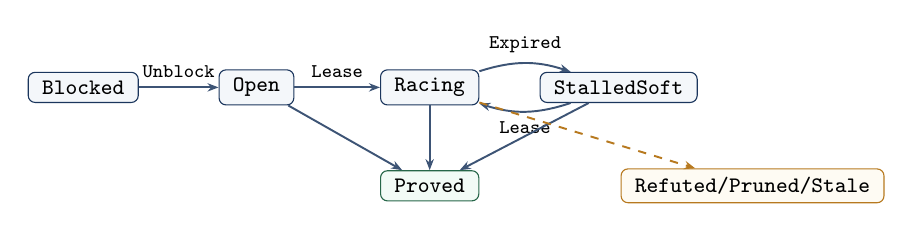
\begin{tikzpicture}[
  x=1cm, y=1cm,
  st/.style={rectangle, rounded corners=2.5pt, draw=NavyBlue, fill=TintNavy, font=\sffamily\footnotesize, inner xsep=5pt, inner ysep=3pt},
  term/.style={rectangle, rounded corners=2.5pt, draw=ForestInk, fill=TintGreen, font=\sffamily\footnotesize\bfseries, inner xsep=5pt, inner ysep=3pt},
  arr/.style={-{Stealth[length=4pt]}, line width=0.7pt, draw=NavyBlue!85}
]
\node[st] (B) at (0, 0) {\code{Blocked}};
\node[st] (O) at (2.2, 0) {\code{Open}};
\node[st] (R) at (4.4, 0) {\code{Racing}};
\node[st] (S) at (6.8, 0) {\code{StalledSoft}};
\node[term] (P) at (4.4, -1.25) {\code{Proved}};
\node[st, draw=AmberInk, fill=TintAmber] (T) at (8.5, -1.25) {\code{Refuted/Pruned/Stale}};

\draw[arr] (B) -- node[above, font=\scriptsize] {\code{Unblock}} (O);
\draw[arr] (O) -- node[above, font=\scriptsize] {\code{Lease}} (R);
\draw[arr] (R) to[bend left=18] node[above, font=\scriptsize] {\code{Expired}} (S);
\draw[arr] (S) to[bend left=18] node[below, font=\scriptsize] {\code{Lease}} (R);
\draw[arr] (O) -- (P);
\draw[arr] (R) -- (P);
\draw[arr] (S) -- (P);
\draw[arr, dashed, draw=AmberInk] (R) -- (T);
\end{tikzpicture}
\caption{\code{quod-core::fsm} 强制执行的核心 \code{TaskState} 状态迁移图。}
\label{fig:fsms}
\end{figure}

\subsection{自动依赖注入、解锁与信息流隔离}
当上游任务 $u$ 的 \code{Proof} 提交通过 Stage~1 并以模块 $m_u$ 并入 $\Truth$ 时，$C_0$ 沿每条依赖边 $(u, w) \in D_{\mathrm{dep}}$ 原子执行：
\begin{enumerate}
  \item $I_w \leftarrow I_w \cup \{m_u\}$（将已过核叠加层注入下游 $w$ 的 \code{curated\_imports}）；
  \item 若 $\forall u' \in \kw{deps}(w),\, s_{u'} = \kw{Proved}$ 且 $s_w = \kw{Blocked}$，则触发 \code{UnblockDependencies} 将 $s_w$ 迁为 \code{Open} 并发射 \code{TaskUnlocked} 事件。
\end{enumerate}

\paragraph{信息流投影隔离。}
为阻断跨时间尺度的上下文污染，$C_1$ 向 $I_1$ 暴露一个过滤掉原始编译器噪声的有损投影：
\[
\pi_{\mathrm{digest}} : (\Truth, \Orch, \Events) \to \kw{WakeupDigest},
\]
仅包含路线摘要、阻塞/开放/停滞计数、高 \code{VOI} 候选节点与卡点告警。原始 Lean 报错栈被路由至 $E_0$ 的 \code{Graveyard} 专供后续尝试同一任务的 $I_0$ Worker 避坑，绝不倾倒入 $I_1$ 上下文。同时，$C_1$ 提供纯函数库 \code{quod-algo}（\code{voi\_rank} 按 $(1-p)\cdot\kw{prio}\cdot(1+0.5\cdot\kw{unblocks})/c$ 排序、跨谱系 \code{detect\_stalls}、\code{check\_coupling} 与 \code{mine\_reusable\_overlays}）。在战略层，审计者 $I_2\text{-A}$ 与提案者 $I_2\text{-B}$ 亦实行上下文隔离，以防范规范空真（Vacuous Truth）。

\subsection{事件溯源编排的元理论}

\begin{theorem}[事件重放确定性与真值单调性定理]\label{thm:replay}
设 $\Events = [e_1, \dots, e_k]$ 是从 $\Sigma_0$ 出发由合法 \code{GraphIrOp} 与核验迁移生成的只追加事件日志，则物化投影重放 $\llbracket \Events \rrbracket(\Sigma_0)$ 是确定的；且对同一纪元内任意前缀 $\Events_1 \preceq \Events_2$，恒有 $\Truth(\Events_1) \sqsubseteq \Truth(\Events_2)$。
\end{theorem}

\begin{proof}
每个状态机迁移函数（\code{EpochState::\-transition}、\code{TaskState::\-transition}、\code{SubmissionState::\-transition}）均为枚举类型上的确定性函数，而 \code{ApplyIrRequest} 按列表顺序确定性地执行 \code{GraphIrOp} 构造子。在 $\Truth$ 中，仅有 \code{DefOverlayVerified} 与 \code{Proof} 验收会向 \code{overlays} 插入新键 $(pid, e, m)$，同一纪元内不存在删除或覆写已入库叠加层的迁移。因此对所有前缀必有 $\Truth(\Events_1) \sqsubseteq \Truth(\Events_2)$。
\end{proof}

\begin{theorem}[合并任务依赖注入完备性定理]\label{thm:merge-unlock}
每当 \code{Merge} 任务 $w$ 通过 \code{Unblock\-Dependencies} 从 \code{Blocked} 迁移至 \code{Open} 时，其所有前置依赖模块 $\{m_u \mid (u, w) \in D_{\mathrm{dep}}\}$ 必已存在于 $\Truth$ 中，且已被注入 $w$ 的 \code{curated\_\-imports} $I_w$。
\end{theorem}

\begin{proof}
因为 $D_{\mathrm{dep}}$ 无环且每个上游任务 $u$ 至多迁移到终态 \code{Proved} 一次（\Cref{fig:fsms}），$u$ 过核时执行的 \code{record\_\-verification\_\-outcome}（\code{memory.rs:2202--2251}）会原子地将 $m_u$ 插入 $\Truth$、将 $m_u$ 追加至下游 $w$ 的 $I_w$，并仅在 \code{all\_\-dependencies\_\-proved} 为真时触发 \code{Unblock\-Dependencies}。故解锁时刻全部前置叠加层均已过核入库且被 $w$ 正确导入。
\end{proof}

% =========================================================
\section{系统实现与架构扩展}\label{sec:impl}
% =========================================================

第~\ref{sec:mech-a} 至~\ref{sec:mech-c} 节形式化的机制已完整实现于六个 Rust crate 中：\code{quod-core}（RBAC、状态机、\code{GraphIrOp}、\code{quod-algo} 与评估器特征）、\code{quod-store}（支持离线构建的 PostgreSQL~16 运行时 \code{sqlx::query} 存储、内存存储与内容寻址 Blob 存储）、\code{quod-sandbox}（Stage~0、最小导入检查、\code{AuditHarness} 渲染与 \code{BwrapRunner}）、\code{quod-verifier}（有界并发核验守护进程）、\code{quod-hub}（Axum HTTP API、\code{/JOIN.md}、\code{/skills/*} 与公开门户）以及 \code{quod-cli}（内嵌角色 Skill 的单二进制工具）。多项目通过 \code{bwrap} 共享只读 \code{toolchain\_bundles}（如 7.4\,GB 的 Mathlib4 \code{v4.36.0}），同时物理隔离各自的 \code{accepted\_\-olean/\-<project\_id>/\-epoch\_<E>/}。

\paragraph{防踩踏分派与悬赏经济。}
$C_0$ 支持双模接单：既允许 Worker 按悬赏和难度门槛自由选单，也支持按 \code{WeightedVoi}、\code{LineageDiversity}、\code{TierMatched} 或 \code{PriorityQueue} 自动撮合，并受 \code{racer\_cap\_k}、跨谱系多样性惩罚与单 Actor 活跃租约上限保护。未显式指定悬赏时，通过纯函数 \code{compute\_\-default\_\-bounty(\-expected\_cost\_c,\; priority,\; failed\_attempts)} 在 $[10, 5000]$ 内确定性定价。

\paragraph{架构扩展模块说明。}
\code{docs/architecture.md} 中还规划了两项尚未作为完整运行时服务落地的扩展能力，本文在此明确区分：
（i）\textbf{L5 常量可达性剪枝与前缀可编译 Git 重放}（\code{quod export}），目前在 \code{lean-harness/\-SliceExtractor.lean} 中具备传递依赖遍历骨架，用于在主定理证毕后剔除死路与废稿，按依赖拓扑重放为每笔提交皆可独立 \code{lake build} 的署名仓库；
（ii）\textbf{M4 \code{quod-evaluator}}，一个常驻无状态统计服务（当前由 \code{quod-core::\-evaluator} 中的 \code{CapabilityEvaluator} 特征预留接口），用于回放 \code{events} 与 \code{Canary} 锚点题，基于无偏 \code{propensity\_score} 遥测运行 Online-IRT / Bradley--Terry 能力与难度重校准。

% =========================================================
\section{相关工作与结语}\label{sec:related}
% =========================================================

\paragraph{小内核验证与协作式 Lean 形式化。}
LCF~\cite{gordon1979edinburgh} 开创了将极小可信内核与可扩展策略层隔离的传统；Lean~4~\cite{demoura2021lean4} 以独立类型检查内核与 \code{collectAxioms} 审计延续了这一范式。围绕 Mathlib~\cite{mathlib2020} 的大型协作形式化工程广泛采用 \code{leanblueprint}~\cite{massot2024blueprint} 可视化依赖蓝图，但其本身不提供面向多智能体并发的 Stage~0/1 隔离核验、闭合 $\Prop$ 竞速边界及事件溯源悬赏市场。

\paragraph{智能体证明器与可信基础设施。}
当代 LLM 证明智能体普遍将搜索策略与 Lean 编译紧耦合在单一 Harness 中。\textsc{Quod} 则反转了这一设计：将全部 LLM 移出 $\Cinfra$，正交解耦真值（$\Truth$）与编排（$\Orch$），并以分层内核审计约束闭合 $\Prop$ 任务，从而使开放的异构人机群体得以高效并发协作，同时永不牺牲基础逻辑可靠性。

\begin{thebibliography}{4}

\bibitem{demoura2021lean4}
Leonardo de Moura and Sebastian Ullrich.
\newblock 2021.
\newblock The Lean 4 Theorem Prover and Programming Language.
\newblock In \emph{Automated Deduction -- CADE 28} (LNCS, Vol. 12699). Springer, 625--635.

\bibitem{gordon1979edinburgh}
Michael J.~C. Gordon, Robin Milner, and Christopher P. Wadsworth.
\newblock 1979.
\newblock \emph{Edinburgh LCF: A Mechanised Logic of Computation}.
\newblock Lecture Notes in Computer Science, Vol. 78. Springer.

\bibitem{mathlib2020}
The mathlib Community.
\newblock 2020.
\newblock The Lean Mathematical Library.
\newblock In \emph{Proceedings of the 9th ACM SIGPLAN International Conference on Certified Programs and Proofs (CPP '20)}. ACM, 367--381.

\bibitem{massot2024blueprint}
Patrick Massot.
\newblock 2024.
\newblock Lean Blueprint: Formalization Planning and Dependency Visualization for Lean 4.
\newblock Software and documentation, \url{https://github.com/PatrickMassot/leanblueprint}.

\end{thebibliography}

\end{document}
